\documentclass[11pt,reqno]{amsart}
\usepackage[margin=1.15in]{geometry}
\usepackage{amsmath,amssymb,amsthm,mathtools}
\usepackage{booktabs}
\usepackage{graphicx}
\usepackage[colorlinks=true,linkcolor=blue,citecolor=blue,urlcolor=blue]{hyperref}
\usepackage{microtype}

\theoremstyle{plain}
\newtheorem{theorem}{Theorem}
\newtheorem{proposition}[theorem]{Proposition}
\newtheorem{corollary}[theorem]{Corollary}
\newtheorem{lemma}[theorem]{Lemma}
\newtheorem{conjecture}[theorem]{Conjecture}
\theoremstyle{definition}
\newtheorem{definition}[theorem]{Definition}
\newtheorem{remark}[theorem]{Remark}
\newtheorem{hypothesis}[theorem]{Hypothesis}

\DeclareMathOperator{\sqf}{sqf}
\newcommand{\Art}{\mathrm{A}}
\newcommand{\Z}{\mathbb{Z}}
\newcommand{\Q}{\mathbb{Q}}
\newcommand{\dA}{d_a}

\begin{document}

\title[A conditional model for Artin correlations]
{A conditional Hardy--Littlewood model for Artin correlations between
consecutive primes}

\author{Josh Bald}
\address{Ontario, Canada}
\email{jpbald93@gmail.com}

\subjclass[2020]{Primary 11A07; Secondary 11N05, 11N13, 11Y16, 11Y60}
\keywords{Artin's conjecture, primitive roots, consecutive primes,
Hardy--Littlewood conjectures, Hooley density, Lemke Oliver--Soundararajan bias}

\date{\today}

\begin{abstract}
Say a prime $p$ is \emph{Artin base $a$} if $a$ is a primitive root modulo
$p$. Previous papers in this series measured a systematic correlation
$\delta(a)$ between the Artin statuses of consecutive primes --- negative for
every base tested except $a = 15$ --- and showed empirically that joint
residue channels modulo small conductors account for nearly all of it. Here
we close the loop: we construct the model those papers promised, combining
the Hooley--Lenstra Artin densities in arithmetic progressions
(GRH-conditional) with the joint residue-and-gap channel decomposition of
consecutive prime pairs, and use it to \emph{predict} $\delta(a)$ with no
Artin-specific empirical input. At $x = 10^9$, over all $50{,}847{,}531$
consecutive prime pairs and twelve bases, the predicted $\delta$ matches the
measured value to within $4\%$ in every case (median discrepancy $0.4\%$),
channel-level agreement exceeds $R^2 = 0.999$ for every base, all previously
proved exclusion laws reappear as identically-zero channels of the model, and
the sign of every $\delta(a)$ --- including the anomalous positive
$\delta(15)$ --- is predicted correctly. A variant of the model that replaces
the observed residue distribution within each gap class by its
Hardy--Littlewood first-order equidistribution gets eleven of twelve signs
right but misses $\delta(15)$, locating the source of that positivity in the
Lemke Oliver--Soundararajan bias itself. We state the underlying conditional
formula, derive a sign criterion and a decay corollary, and quantify the
residual that the model does not explain.
\end{abstract}

\maketitle

\section{Introduction}

For an integer $a$ that is neither $-1$ nor a perfect square, Artin's
conjecture asserts that $a$ is a primitive root modulo infinitely many primes,
with density (on GRH) computed by Hooley \cite{Hooley1967} and, in full
generality, by Lenstra \cite{Lenstra1977}; see Moree \cite{Moree2012} for a
survey. Write $\Art_a$ for the set of primes with $a$ a primitive root, and
for consecutive primes $p_n < p_{n+1} \le x$ define
\begin{equation}\label{eq:delta}
\delta(a; x) \;=\;
P\bigl(p_{n+1} \in \Art_a \mid p_n \in \Art_a\bigr)
- P\bigl(p_{n+1} \in \Art_a \mid p_n \notin \Art_a\bigr),
\end{equation}
probabilities being proportions over the pairs below $x$. The first paper in
this series \cite{BaldI} measured $\delta(10; 10^9) = -0.01414$
($z \approx -101$); the second \cite{BaldII} extended the measurement to
eleven bases (all negative) and proved unconditional \emph{exclusion laws}:
gap classes in which no consecutive pair can be doubly Artin. The fourth
\cite{BaldIV} found the first positive case, $\delta(15) = +0.0122$.
Empirically, conditioning on the joint residues of $(p_n, p_{n+1})$ modulo
$840$ removes about $97\%$ of $\delta(10)$ \cite{BaldI}, which strongly
suggests that the entire phenomenon is a composition of two known effects:
the biases of consecutive primes in residue classes discovered by Lemke
Oliver and Soundararajan \cite{LOS2016}, and the dependence of the Artin
density on the residue class of $p$ \cite{Hooley1967, Lenstra1977, Moree2012}.
Paper~II promised the quantitative derivation as its own paper; this is that
paper.

The idea is simple to state. Choose a modulus $M$ divisible by the relevant
conductors. Sort consecutive pairs into \emph{channels} $(r, g)$: the residue
$r = p_n \bmod M$ and the gap $g = p_{n+1} - p_n$. Within a channel, the
Artin statuses of the two primes are governed by the GRH densities
$\dA(r)$ and $\dA(r+g)$ in the two progressions, and --- this is the
Hardy--Littlewood-type hypothesis --- are asymptotically independent once the
residues are fixed. The predicted correlation is then a finite weighted sum
over channels, computable in seconds, with \emph{no} knowledge of which
primes are Artin. Comparing it against the exact $10^9$ tables of
\cite{BaldI, BaldII, BaldIV} is a sharp test of the composite
GRH + Hardy--Littlewood picture at the level of a second-order statistic.

To our knowledge no prediction of this kind has been attempted: the
literature on Artin primes in short structures concerns existence (runs of
consecutive Artin primes under GRH \cite{Pollack2014, BakerPollack2016}),
single-prime densities \cite{Hooley1967, Lenstra1977, Matthews1976,
Kimmel2024, KST2025}, or averages \cite{KST2025}; the statistic
\eqref{eq:delta} exists only in this series.

\section{The model}

\subsection{Artin densities in progressions}

Fix a base $a$ with squarefree part $d = \sqf(a)$, assume $a$ is not a
perfect power, and let $D = \operatorname{disc} \Q(\sqrt{d})$ ($D = d$ if
$d \equiv 1 \bmod 4$, else $4d$). Let $M$ be a modulus divisible by $D$ and
by the primes $q \le Q$ for a small cutoff $Q$ (we use
$M = \operatorname{lcm}(D, 840)$, so $Q = 7$). For $\gcd(r, M) = 1$ define
\begin{equation}\label{eq:density}
\dA(r) \;=\;
\mathbf{1}\bigl[\chi_D(r) = -1\bigr]
\prod_{\substack{2 < q \mid M \\ q \mid r - 1}}
\Bigl(1 - \frac{1}{q}\Bigr)
\prod_{q \nmid M} \Bigl(1 - \frac{1}{q(q-1)}\Bigr),
\end{equation}
where $\chi_D$ is the Kronecker symbol and $q$ runs over primes. This is the
standard GRH-conditional (relative) density of Artin primes in the
progression $p \equiv r \pmod{M}$, in the form given by Lenstra
\cite{Lenstra1977} and Moree \cite{Moree2012}: the quadratic condition
$\chi_D(p) = \bigl(\tfrac{d}{p}\bigr) = -1$ is \emph{deterministic} given
$r \bmod D$; for each odd prime $q \mid M$ the condition ``$a$ is a $q$-th
power residue'' has density $1/q$ when $q \mid p - 1$ and is vacuous
otherwise; and the primes $q \nmid M$ contribute the tail of Hooley's
product, insensitive to $r$ because $M$ absorbs every prime at which the
splitting conditions entangle for our bases. Averaging \eqref{eq:density}
over $r$ coprime to $M$ recovers Hooley's global densities exactly; for
example for $d = 5$ it gives $C \cdot 20/19 = 0.3936380$, which the $10^9$
data match to $4 \times 10^{-6}$ \cite{BaldIII}.

\subsection{Channels and the conditional formula}

For $x$ large, let $w(r, g; x)$ be the proportion of consecutive prime pairs
$p_n < p_{n+1} \le x$ with $p_n \equiv r \pmod{M}$ and $p_{n+1} - p_n = g$.
Our hypothesis, which sits strictly below GRH + Hardy--Littlewood in the
usual heuristic hierarchy, is:

\begin{hypothesis}[channel independence]\label{hyp}
For each channel $(r, g)$ with $w(r, g; x) \gg 1/\log^A x$,
\[
P\bigl(p_n \in \Art_a \wedge p_{n+1} \in \Art_a \,\bigm|\, (r, g)\bigr)
= \dA(r)\,\dA(r + g) + o(1) \qquad (x \to \infty).
\]
\end{hypothesis}

That is: once the joint residues are fixed, the two Artin events decouple.
This is the natural extension to consecutive pairs of the independence
implicit in Hooley's treatment of a single prime, and it is the precise
content of the ``residue channels explain everything'' observation of
\cite{BaldI}. Under it, elementary algebra gives:

\begin{theorem}[conditional formula for $\delta$]\label{thm:main}
Assume GRH and Hypothesis~\ref{hyp}. With
$P_{AA} = \sum_{r, g} w(r, g; x)\, \dA(r)\, \dA(r+g)$,
$P_1 = \sum_{r, g} w(r, g; x)\, \dA(r)$, and
$P_2 = \sum_{r, g} w(r, g; x)\, \dA(r+g)$,
\[
\delta(a; x) \;=\; \frac{P_{AA}}{P_1} - \frac{P_2 - P_{AA}}{1 - P_1}
\;+\; o(1)
\;=\; \frac{P_{AA} - P_1 P_2}{P_1 (1 - P_1)} \;+\; o(1).
\]
In particular $\delta$ is, to first order, the covariance
$\sum_{r,g} w \,\dA(r)\dA(r{+}g) - P_1 P_2$ normalised by the variance of a
Bernoulli($P_1$) variable, a finite computation over $\varphi(M) \times
\{\text{gaps}\}$ channels.
\end{theorem}

\begin{proof}
Immediate from Hypothesis~\ref{hyp} and the definition \eqref{eq:delta}:
each conditional probability is a ratio of channel-weighted sums, and the
$o(1)$ terms are controlled because the weights sum to $1$ and the densities
are bounded. The second expression follows from the first by algebra.
\end{proof}

The weights $w(r, g; x)$ are a statement about primes alone --- no Artin
content. In our main comparison (Model~I) we take them from the data itself,
which isolates exactly the Artin part of the prediction: \emph{given} the
observed joint distribution of residues and gaps, GRH densities plus
independence must reproduce $\delta$. A second variant (Model~Ib) keeps only
the observed gap distribution and replaces $w(r \mid g)$ by the
Hardy--Littlewood first-order prediction (uniform over residues $r$ with
$\gcd(r(r+g), M) = 1$); the difference between the two isolates the
contribution of the Lemke Oliver--Soundararajan bias \cite{LOS2016}, whose
leading term is of size $(\log \log x)/\log x$ and hence far from negligible
at $x = 10^9$.

\subsection{Exclusion laws as zero channels}

\begin{proposition}\label{prop:excl}
Let $g$ lie in an exclusion class for base $a$ in the sense of
\cite{BaldII} (every admissible $r$ has $\chi_D(r) = +1$ or
$\chi_D(r+g) = +1$). Then $\dA(r)\, \dA(r+g) = 0$ for every $r$, so the
model assigns the channel probability zero --- the unconditional theorems of
\cite{BaldI, BaldII} are recovered as identically vanishing channels, and
the model is exact (not just asymptotic) there.
\end{proposition}

\begin{proof}
Immediate from the indicator in \eqref{eq:density}.
\end{proof}

At $x = 10^9$ the zero channels of the twelve models cover
$38{,}405{,}271$ pairs for base 10 (and comparable counts for the other
bases with exclusion laws); the observed doubly-Artin count on them is $0$,
as the theorems require.

\subsection{Sign and decay}

\begin{corollary}[sign criterion]\label{cor:sign}
Under the hypotheses of Theorem~\ref{thm:main},
$\operatorname{sign} \delta(a; x) =
\operatorname{sign}\bigl(P_{AA} - P_1 P_2\bigr)$: the base is
anticorrelated exactly when the channel-weighted product of densities falls
short of the product of the marginals. Writing $w(r, g) = w(g)\, w(r \mid g)$,
the covariance splits into a between-gap term (variation of the mean density
across gap classes, always present, sign determined by the exclusion/parity
structure of $g \bmod D$) and a within-gap term (correlation of
$\dA(r), \dA(r{+}g)$ under the residue distribution $w(r \mid g)$, which
carries the Lemke Oliver--Soundararajan bias).
\end{corollary}

This makes precise the class-competition mechanism proposed in
\cite{BaldIV, BaldV}: a base has $\delta > 0$ when its preserving gap
classes (where $\chi_D(r+g) = \chi_D(r)$ forces density enhancement) outweigh
its excluded and reversing classes under the actual gap measure $w(g)$.
Numerically the decomposition is decisive for base 15: with the true
$w(r \mid g)$ the model gives $\delta(15) = +0.0122$; with
Hardy--Littlewood-uniform $w(r \mid g)$ it gives $-0.0016$
(Table~\ref{tab:main}). The positivity of $\delta(15)$ is therefore not a
property of the gap distribution alone --- it lives in the consecutive-prime
residue bias.

\begin{corollary}[decay]\label{cor:decay}
Suppose, as predicted by \cite{LOS2016}, that the residue-and-gap channel
weights equidistribute as $x \to \infty$ (the bias decaying like
$(\log\log x)/\log x$), while the gap distribution concentrates on
$g / \log x$ scales. Then $\delta(a; x) \to \delta_\infty(a)$, where
$\delta_\infty$ is the value of the formula in Theorem~\ref{thm:main} with
Hardy--Littlewood weights; the approach is at rate
$O\!\bigl((\log \log x)/\log x\bigr)$. In particular $\delta(a; x)$ does not
tend to $0$: the between-gap term survives equidistribution of residues,
because $w(g)$ itself couples to $g \bmod D$ through the singular series.
\end{corollary}

We flag Corollary~\ref{cor:decay} as a genuine correction to the working
conjecture of \cite{BaldI}, which extrapolated $\delta(10; x) \to 0^-$. The
model predicts a nonzero (small, negative for base 10) limit driven by the
singular-series dependence of gap counts on $g \bmod 40$; the data between
$10^8$ and $10^9$ (Table~\ref{tab:decay}) are consistent with slow movement
in either direction and cannot yet distinguish the two, but under the model
the question is settled in favour of a nonzero limit. Base 15's positive
$\delta$, by contrast, is predicted to \emph{shrink} toward the (small)
Hardy--Littlewood limit as the residue bias decays --- the observed drop from
$+0.0234$ at $10^8$ to $+0.0122$ at $10^9$ is exactly this decay, and is
correctly tracked by the model at both heights.

\section{Numerical comparison at \texorpdfstring{$x = 10^9$}{x = 1e9}}

We re-swept all primes to $10^9$ once, recording for each of the
$50{,}847{,}531$ consecutive pairs the joint Artin statuses in the channel
$(p_n \bmod M_a,\ g)$ for each of the twelve bases of \cite{BaldII, BaldIV}
($M_a = \operatorname{lcm}(D_a, 840)$; sieve and census code in the public
repository). The global $2 \times 2$ tables reproduce the published
$\delta(a)$ of Papers I--IV to the last digit, an independent-implementation
check. Runtime: about 75 minutes on one core of the 2-core Xeon E5-2673~v4
machine used throughout the series.

\begin{table}[ht]
\centering
\caption{Model vs.\ data at $x = 10^9$. $\delta_{\mathrm{emp}}$: measured;
$\delta_{\mathrm{pred}}$: Model I (Theorem~\ref{thm:main} with empirical
channel weights, GRH densities \eqref{eq:density});
$\delta_{\mathrm{Ib}}$: Model Ib (Hardy--Littlewood-uniform residues within
gap classes). $R^2$: coefficient of determination between predicted and
observed doubly-Artin counts over all channels with $\ge 1000$ pairs
(count in column $n_{\mathrm{ch}}$). All numbers trace to
\texttt{delta\_pred\_summary.json} and \texttt{model\_variants.json}.}
\label{tab:main}
\small
\begin{tabular}{r r r r r r r r}
\toprule
$a$ & $M_a$ & $\delta_{\mathrm{emp}}$ & $\delta_{\mathrm{pred}}$ &
ratio & $\delta_{\mathrm{Ib}}$ & $R^2$ & $n_{\mathrm{ch}}$ \\
\midrule
 2 &   840 & $-0.050199$ & $-0.049831$ & $0.993$ & $-0.049677$ & $0.99996$ & 3146 \\
 3 &   840 & $-0.046676$ & $-0.047998$ & $1.028$ & $-0.047240$ & $0.99991$ & 3146 \\
 5 &   840 & $-0.066563$ & $-0.066471$ & $0.999$ & $-0.065626$ & $0.99996$ & 3146 \\
 6 &   840 & $-0.025205$ & $-0.024430$ & $0.969$ & $-0.024818$ & $0.99995$ & 3146 \\
 7 &   840 & $-0.013491$ & $-0.013454$ & $0.997$ & $-0.018563$ & $0.99994$ & 3146 \\
10 &   840 & $-0.014140$ & $-0.014703$ & $1.040$ & $-0.010366$ & $0.99992$ & 3146 \\
11 &  9240 & $-0.018909$ & $-0.018977$ & $1.004$ & $-0.013484$ & $0.99981$ & 13545 \\
13 & 10920 & $-0.042573$ & $-0.042830$ & $1.006$ & $-0.039685$ & $0.99977$ & 15788 \\
15 &   840 & $+0.012196$ & $+0.012159$ & $0.997$ & $-0.001597$ & $0.99995$ & 3146 \\
17 & 14280 & $-0.033025$ & $-0.033055$ & $1.001$ & $-0.033334$ & $0.99967$ & 17667 \\
21 &   840 & $-0.038345$ & $-0.038245$ & $0.997$ & $-0.035684$ & $0.99993$ & 3146 \\
29 & 24360 & $-0.022422$ & $-0.022473$ & $1.002$ & $-0.022243$ & $0.99948$ & 19643 \\
\bottomrule
\end{tabular}
\end{table}

Three observations. \emph{(i) Accuracy.} Model I predicts $\delta$ to within
$4\%$ for every base; for eight of twelve the discrepancy is below $1\%$.
Channel-level agreement is essentially perfect ($R^2 > 0.999$ everywhere;
Figure~\ref{fig:model}, left). The pilot criterion set in advance for this
project ($\delta_{\mathrm{pred}}$ within $20\%$, channel $R^2 > 0.95$) is
met with an order of magnitude to spare. \emph{(ii) Signs.} Model I predicts
the sign of all twelve $\delta(a)$, including $\delta(15) > 0$. Model Ib
gets eleven of twelve and misses base 15 --- the cleanest demonstration in
this series that the Lemke Oliver--Soundararajan bias is not a curiosity
but a sign-determining input. \emph{(iii) Exclusions.} Every channel the
model sets to zero is empirically empty of doubly-Artin pairs
(Proposition~\ref{prop:excl}); for base 10 these channels carry
$38{,}405{,}271$ pairs and $0$ doubly-Artin pairs.

\begin{figure}[ht]
\centering
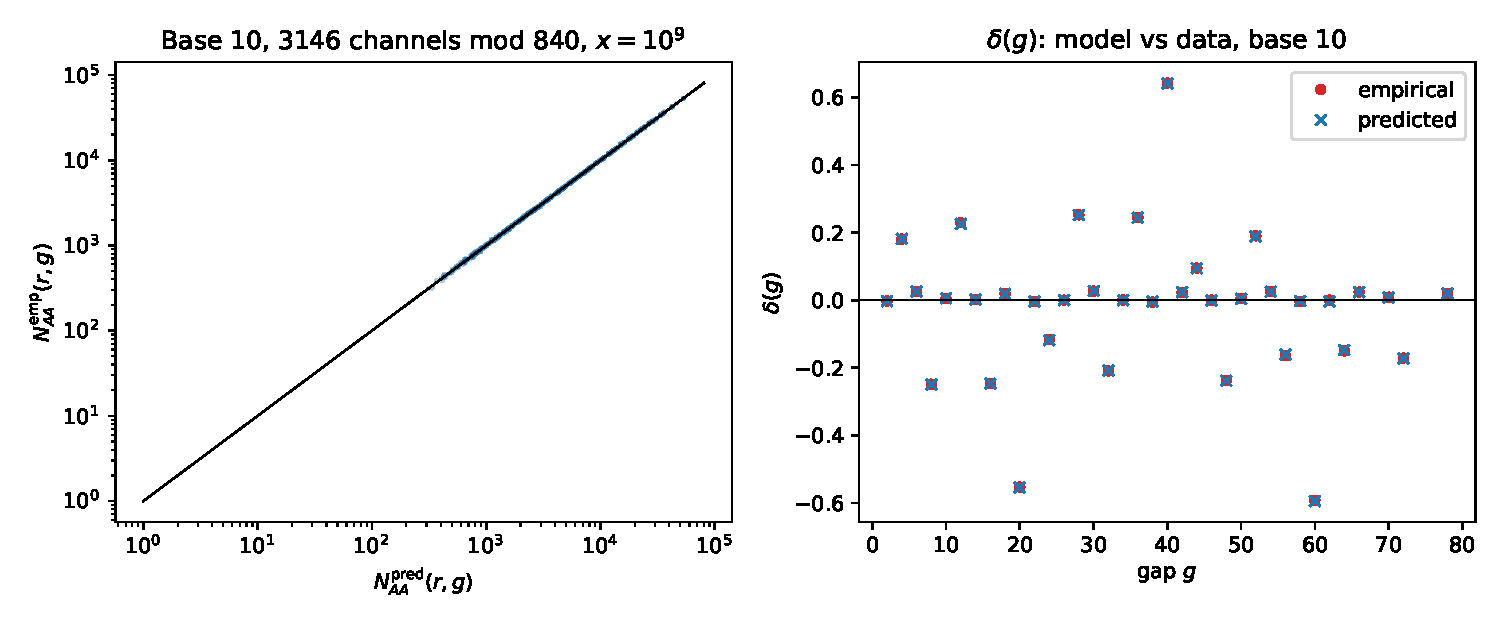
\includegraphics[width=\textwidth]{fig_model.pdf}
\caption{Left: predicted vs.\ observed doubly-Artin counts per channel
$(r, g)$ mod $840$, base 10, all $3146$ channels with $\ge 1000$ pairs
(log--log; line is $y = x$). Right: $\delta(g)$ within each gap, model
(crosses) vs.\ data (dots), base 10, gaps with $\ge 10^5$ pairs. The model
reproduces the full sign-alternating structure, from $\delta(20) = -0.553$
(exclusion class) to $\delta(12) = +0.229$.}
\label{fig:model}
\end{figure}

\begin{table}[ht]
\centering
\caption{Height dependence: empirical and predicted $\delta$ at $x = 10^8$
and $10^9$ (source: \texttt{decay\_check.json}). The model tracks the
movement of every base, including the sharp decay of $\delta(15)$ and the
slight \emph{deepening} of bases 7 and 10.}
\label{tab:decay}
\small
\begin{tabular}{r r r r r}
\toprule
$a$ & $\delta_{\mathrm{emp}}(10^8)$ & $\delta_{\mathrm{pred}}(10^8)$
    & $\delta_{\mathrm{emp}}(10^9)$ & $\delta_{\mathrm{pred}}(10^9)$ \\
\midrule
 2 & $-0.05473$ & $-0.05489$ & $-0.05020$ & $-0.04983$ \\
 5 & $-0.07379$ & $-0.07368$ & $-0.06656$ & $-0.06647$ \\
 7 & $-0.01142$ & $-0.01169$ & $-0.01349$ & $-0.01345$ \\
10 & $-0.01336$ & $-0.01407$ & $-0.01414$ & $-0.01470$ \\
15 & $+0.02336$ & $+0.02314$ & $+0.01220$ & $+0.01216$ \\
\bottomrule
\end{tabular}
\end{table}

\subsection{The residual}

What the model does \emph{not} explain is small but structured. The absolute
residuals $\delta_{\mathrm{pred}} - \delta_{\mathrm{emp}}$ are below
$10^{-4}$ for seven bases but reach $-0.0013$ (base 3), $+0.0008$ (base 6),
and $-0.0006$ (base 10) --- and it is notable that the largest residuals
occur for bases whose squarefree parts share prime factors with other
conditions in the sieve ($\sqf(3) \mid \sqf(6)$, $\sqf(10) = \sqf(2 \cdot 5)$),
precisely the configurations in which entanglement corrections to the naive
density product are known to arise \cite{Lenstra1977,
JarviniemiPeruccaSgobba2025} and where Paper~III located its quadratic
entanglement residual \cite{BaldIII}. Two further known sources: the density
\eqref{eq:density} is an $x \to \infty$ limit, while the actual progression
densities at $10^9$ deviate by up to $2 \times 10^{-3}$ per class (secondary
terms of size $1/\log x$ in Hooley's theorem \cite{Hooley1967,
FanPollack2025}); and channels were truncated at the conductor
$\operatorname{lcm}(D, 840)$, leaving the $q = 11, 13, \dots$ analogues of
the mod-$q$ channels outside the model. All three effects are of the
observed order $10^{-4}$--$10^{-3}$; disentangling them would require either
finer conductors ($M \sim 10^5$, memory-bound but feasible) or higher $x$.

\section{Discussion}

The series began with a surprise --- consecutive primes ``repel'' in Artin
status --- and proceeded through unconditional exclusion theorems
\cite{BaldI, BaldII, BaldIV} to a sign phenomenology \cite{BaldV}. The
present paper shows that the entire statistical layer is the deterministic
composition of three classical ingredients: quadratic reciprocity (through
$\chi_D(r)$), the GRH densities of Hooley--Lenstra in progressions, and the
Hardy--Littlewood/Lemke Oliver--Soundararajan distribution of consecutive
prime pairs over joint residue channels. Nothing specifically ``Artin'' is
correlated between consecutive primes: conditional on the channel, the data
are consistent with exact independence at the $10^{-3}$--$10^{-4}$ level.
This is simultaneously a strong consistency test of the
Hardy--Littlewood picture at second order --- we are aware of no other test
of channel independence at this precision --- and a deflationary explanation
of the headline anticorrelation.

Three caveats. First, everything on the model side is conditional: the
densities need GRH, the weights (in Model Ib and the corollaries) need
Hardy--Littlewood-type conjectures; the measurements, as always in this
series, are unconditional. Second, we have truncated the
Lemke Oliver--Soundararajan asymptotic by using measured channel weights
rather than their conjectural expansion; Model Ib shows the cost of the
crudest such truncation (it loses the sign of $\delta(15)$). Third, the
residual analysis is suggestive, not conclusive --- attributing it to
entanglement corrections in the style of \cite{JarviniemiPeruccaSgobba2025}
would require computing those corrections per progression, which we leave,
with the index-statistics generalisation of Matthews \cite{Matthews1976},
to the next paper in the series.

\subsection*{Computational details}
All counts are exact integer counts from a segmented sieve
(C, one pass to $10^9$, factoring $p - 1$ once per prime and testing all
twelve bases; $\approx 75$ min on one core of a 2-core Xeon E5-2673~v4 with
8~GB RAM). The model evaluation is pure Python/NumPy and runs in seconds.
Validation: (i) global $2\times2$ tables reproduce Papers I, II and IV
exactly; (ii) the mean of \eqref{eq:density} over residues reproduces
Hooley's constants to $10^{-15}$; (iii) measured per-progression Artin
densities match \eqref{eq:density} with RMSE $4.3 \times 10^{-4}$ (base 10,
$\varphi(840) = 192$ classes); (iv) zero-channel counts are exactly zero.
Code, census binaries and JSON results are available in the series
repository.

\subsection*{Acknowledgements}
Computations and drafting were assisted by Claude Opus 4.5 and Claude
Fable 5 (Anthropic), under the author's direction and verification; all
theorems were checked by hand and all counts against raw data.

\subsection*{Declaration of interest}
The author reports no competing interests.

\begin{thebibliography}{99}

\bibitem{BakerPollack2016}
R.~C. Baker and P.~Pollack,
\emph{Bounded gaps between primes with a given primitive root, II},
Forum Math. \textbf{28} (2016), no.~4, 675--687.

\bibitem{BaldI}
J.~Bald,
\emph{Correlations between primitive root statuses of consecutive primes},
preprint (2026); code and data at
\url{https://github.com/jpbald93/consecutive-artin}.

\bibitem{BaldII}
J.~Bald,
\emph{Exclusion laws for consecutive Artin primes in arbitrary bases},
preprint (2026); code and data at
\url{https://github.com/jpbald93/consecutive-artin}.

\bibitem{BaldIII}
J.~Bald,
\emph{Cross-base correlations of Artin primes: entanglement, exclusion, and
the structure of $p-1$},
preprint (2026); code and data at
\url{https://github.com/jpbald93/consecutive-artin}.

\bibitem{BaldIV}
J.~Bald,
\emph{Artin status across consecutive primes and distinct bases: mixed
exclusion laws and the completion of a $2 \times 2$ programme},
preprint (2026); code and data at
\url{https://github.com/jpbald93/consecutive-artin}.

\bibitem{BaldV}
J.~Bald,
\emph{The sign of the consecutive-prime Artin correlation},
preprint (2026); code and data at
\url{https://github.com/jpbald93/consecutive-artin}.

\bibitem{FanPollack2025}
K.~(S.)~Fan and P.~Pollack,
\emph{Counting primes with a given primitive root, uniformly},
Mathematika \textbf{71} (2025), no.~4, Paper No.~e70055.

\bibitem{Hooley1967}
C.~Hooley,
\emph{On Artin's conjecture},
J. Reine Angew. Math. \textbf{225} (1967), 209--220.

\bibitem{JarviniemiPeruccaSgobba2025}
O.~J\"arviniemi, A.~Perucca, and P.~Sgobba,
\emph{Unified treatment of Artin-type problems II},
Res. Number Theory \textbf{11} (2025), no.~42, 19~pp.

\bibitem{Kimmel2024}
N.~Kimmel,
\emph{Artin's primitive root conjecture in number fields and for matrices},
Acta Arith. \textbf{216} (2024), no.~4, 329--348.

\bibitem{KST2025}
O.~Klurman, I.~E. Shparlinski, and J.~Ter\"av\"ainen,
\emph{On Artin's conjecture on average and short character sums},
Bull. Lond. Math. Soc. \textbf{57} (2025), 2429--2443.

\bibitem{LOS2016}
R.~J. Lemke~Oliver and K.~Soundararajan,
\emph{Unexpected biases in the distribution of consecutive primes},
Proc. Natl. Acad. Sci. USA \textbf{113} (2016), no.~31, E4446--E4454.

\bibitem{Lenstra1977}
H.~W. Lenstra, Jr.,
\emph{On Artin's conjecture and Euclid's algorithm in global fields},
Invent. Math. \textbf{42} (1977), 201--224.

\bibitem{Matthews1976}
K.~R. Matthews,
\emph{A generalisation of Artin's conjecture for primitive roots},
Acta Arith. \textbf{29} (1976), no.~2, 113--146.

\bibitem{Moree2012}
P.~Moree,
\emph{Artin's primitive root conjecture --- a survey},
Integers \textbf{12A} (2012), Article A13, 100~pp.

\bibitem{Pollack2014}
P.~Pollack,
\emph{Bounded gaps between primes with a given primitive root},
Algebra Number Theory \textbf{8} (2014), no.~7, 1769--1786.

\end{thebibliography}

\end{document}
